\begin{figure*}[t]
      \subfloat[p0 core3, \bench{daxpy}] {
        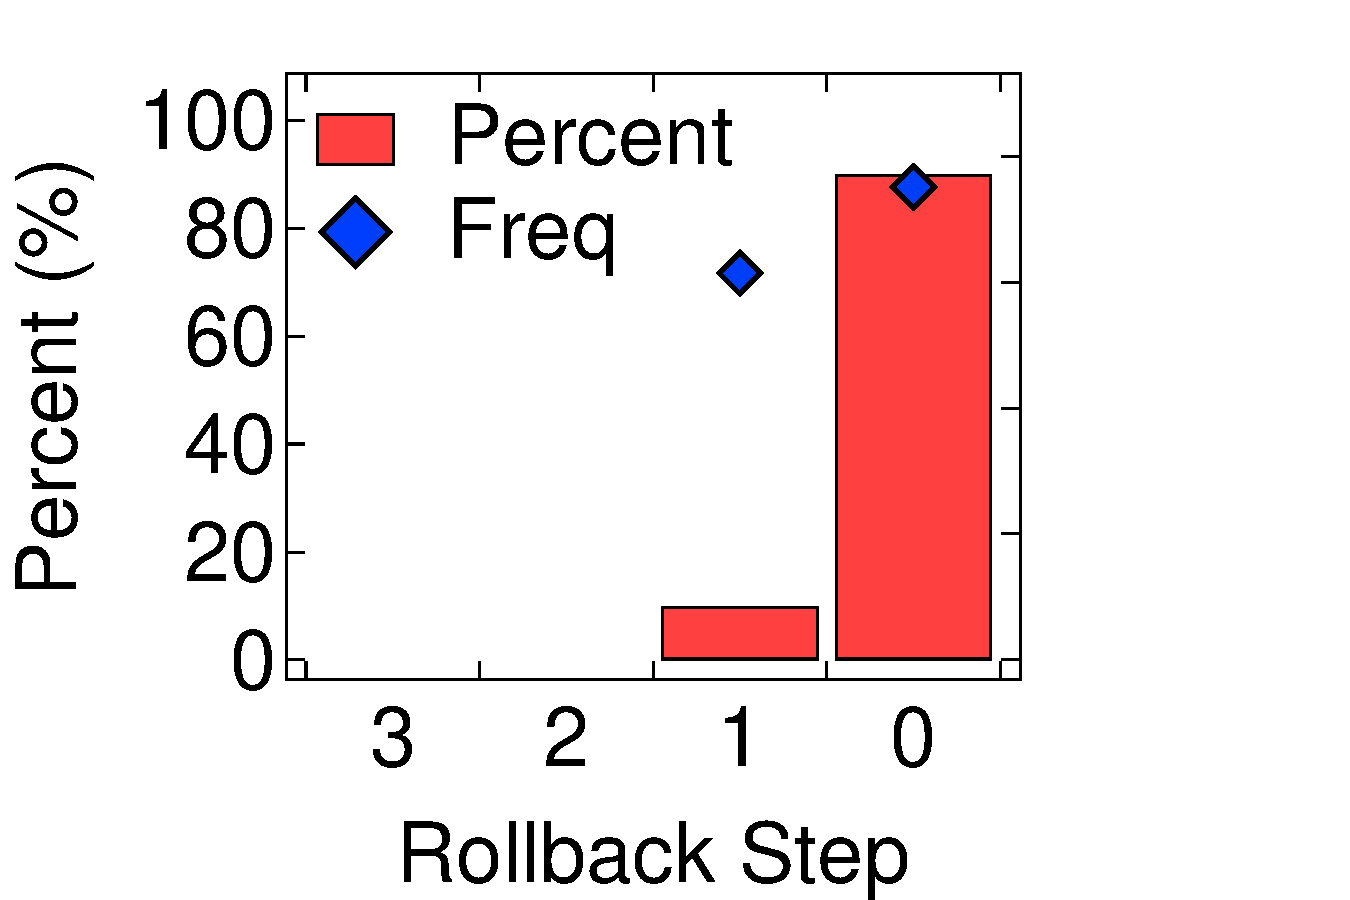
\includegraphics[trim=0 0 0 0,clip,width=.3\linewidth]{graphs/process/ubench-limit-dist/fp-limit-dist-p0c3.pdf}
      }
      \hfill
      \subfloat[p0 core4, \bench{daxpy}] {
        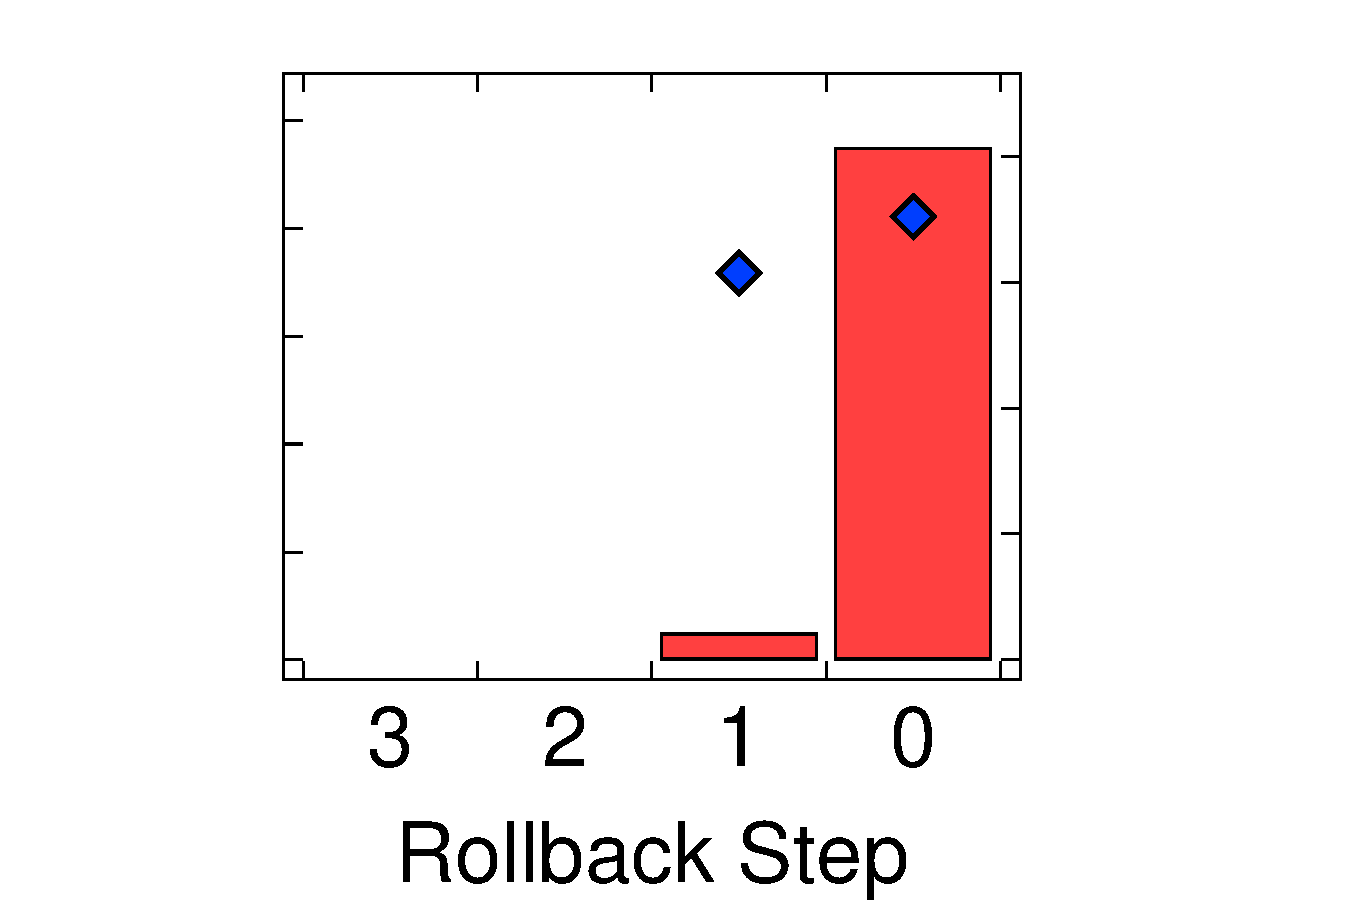
\includegraphics[trim=0 0 0 0,clip,width=.3\linewidth]{graphs/process/ubench-limit-dist/fp-limit-dist-p0c4.pdf}
      }
      \hfill
      \subfloat[p1 core3, \bench{stream}] {
        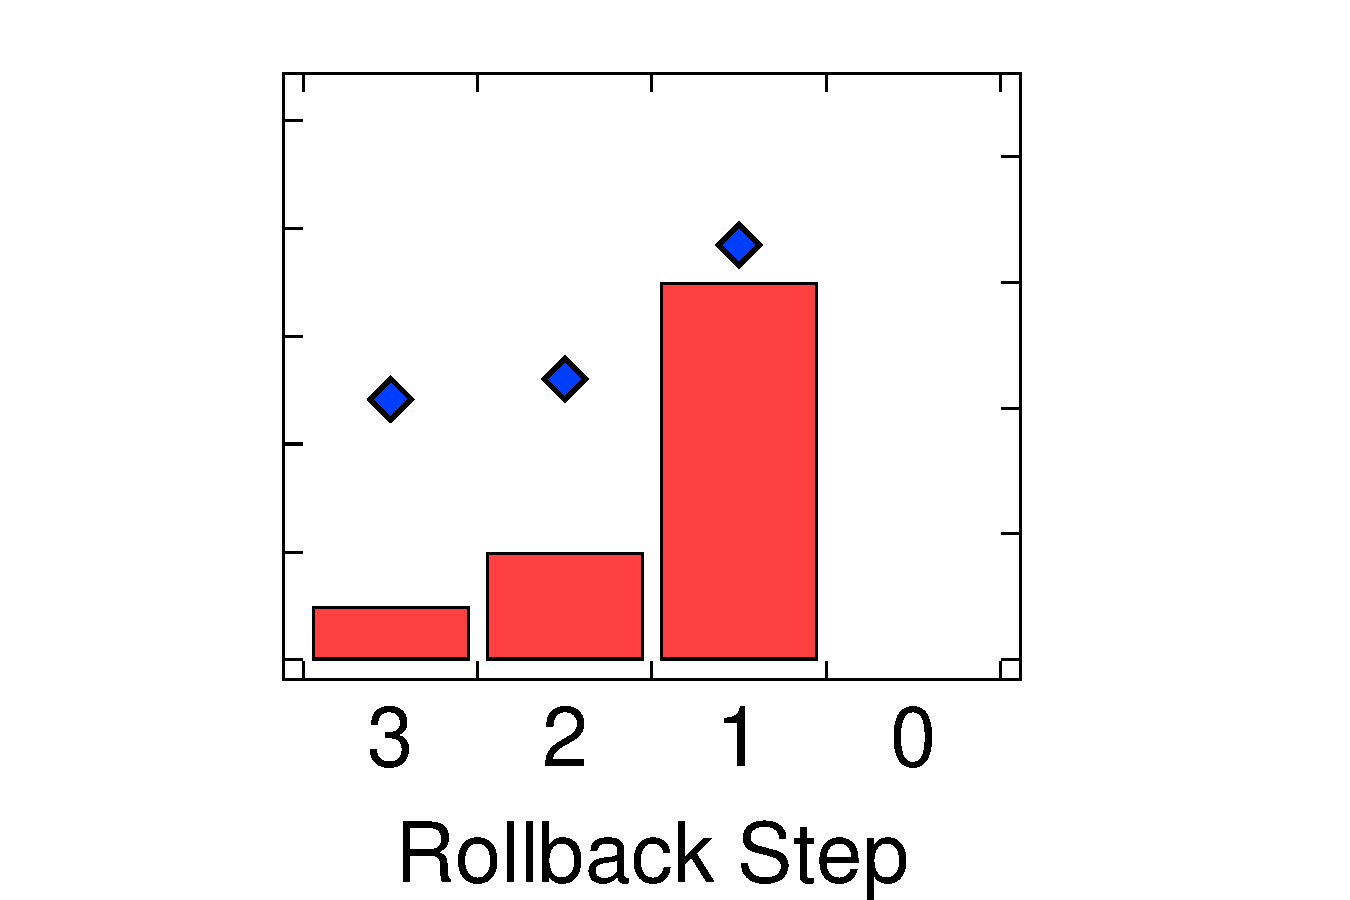
\includegraphics[trim=0 0 0 0,clip,width=.3\linewidth]{graphs/process/ubench-limit-dist/mem-limit-dist-p1c3.pdf}
      }

      \subfloat[p1 core4, \bench{stream}] {
        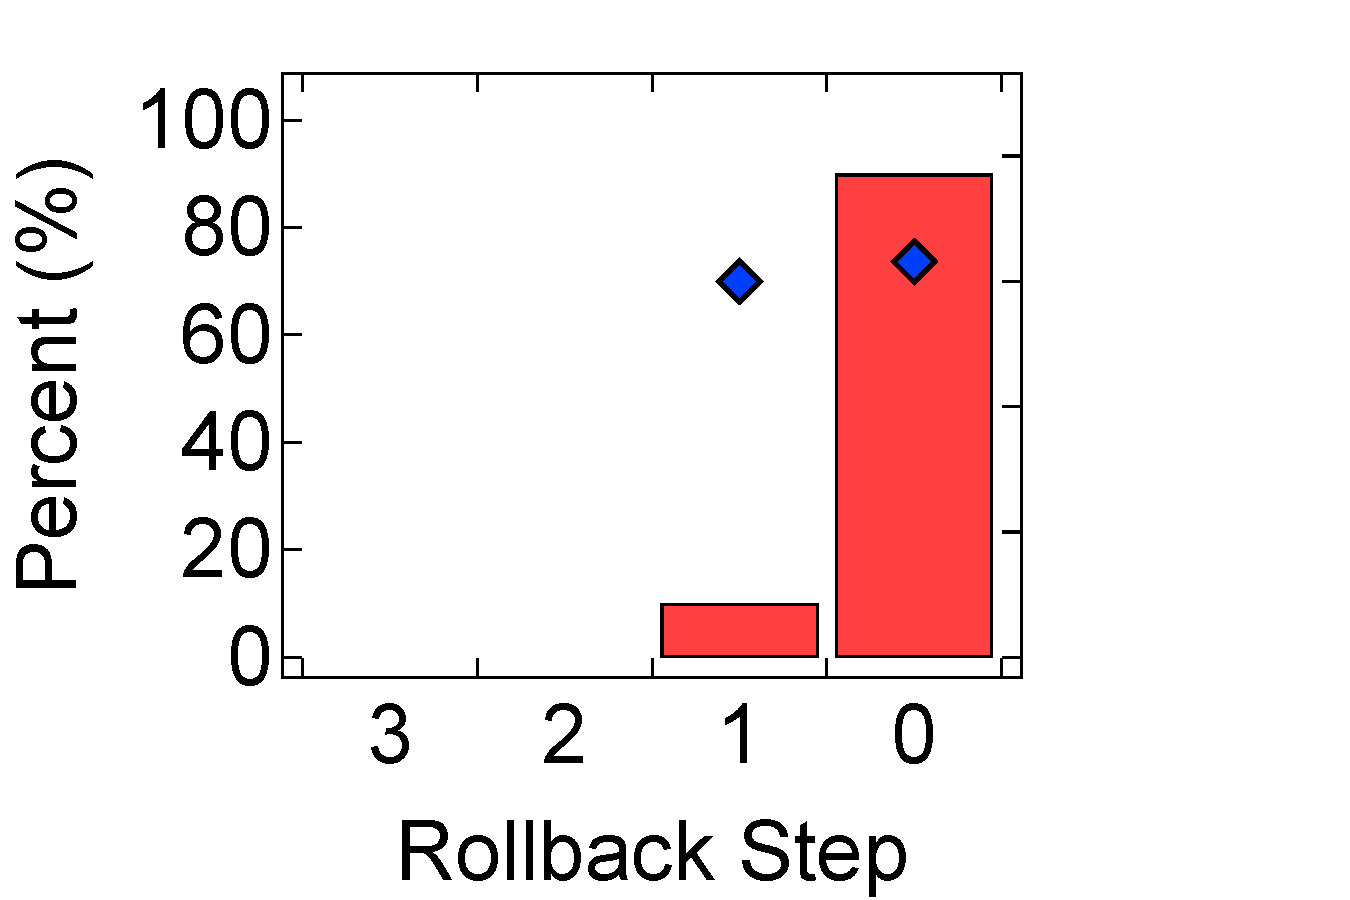
\includegraphics[trim=0 0 0 0,clip,width=.3\linewidth]{graphs/process/ubench-limit-dist/mem-limit-dist-p1c4.pdf}
      }
      \hfill
      \subfloat[p1 core5, \bench{coremark}] {
        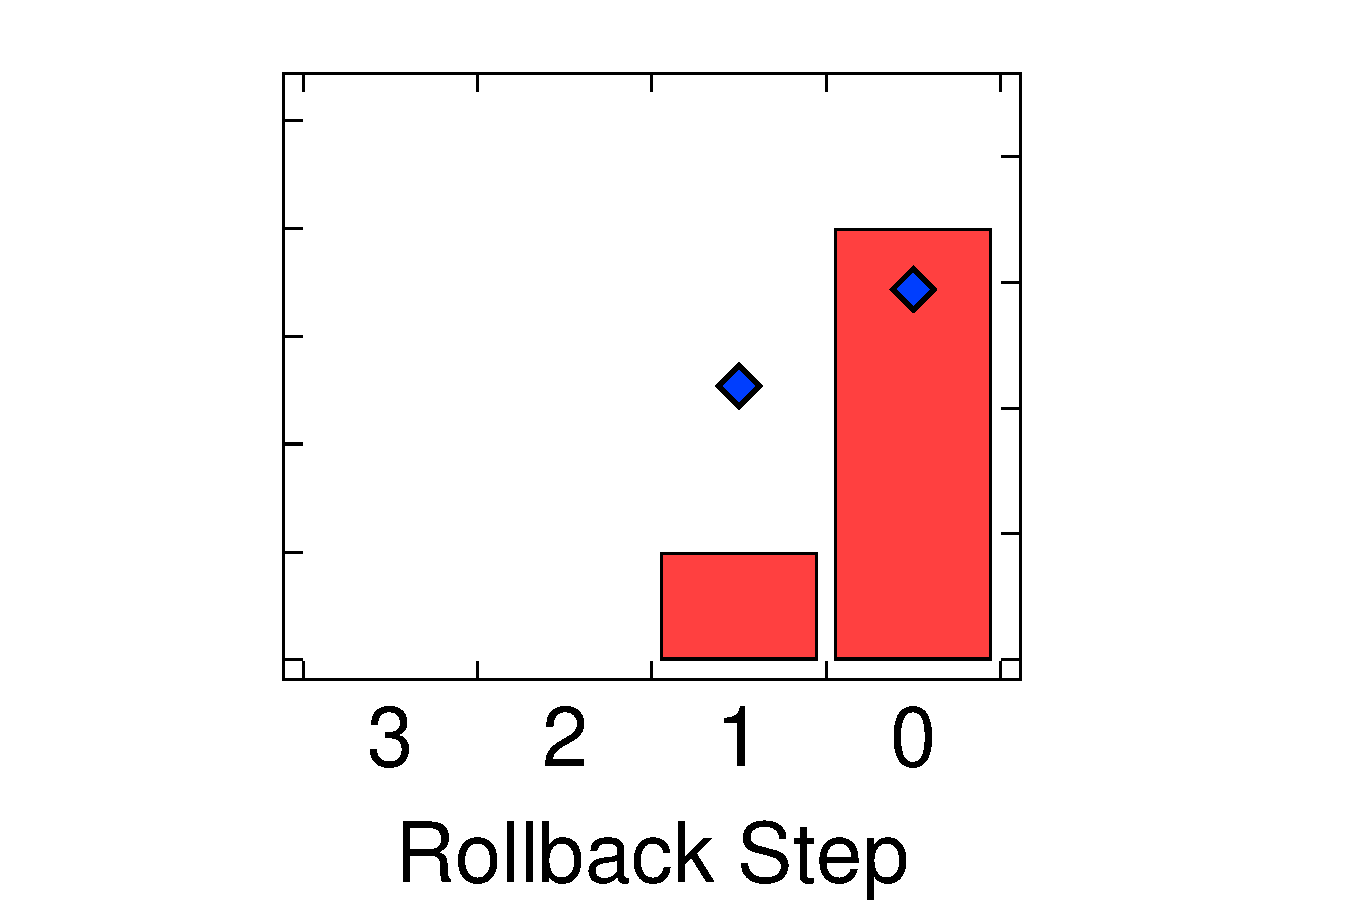
\includegraphics[trim=0 0 0 0,clip,width=.3\linewidth]{graphs/process/ubench-limit-dist/int-limit-dist-p1c5.pdf}
      }
      \hfill
      \subfloat[p1 core7, \bench{coremark}] {
        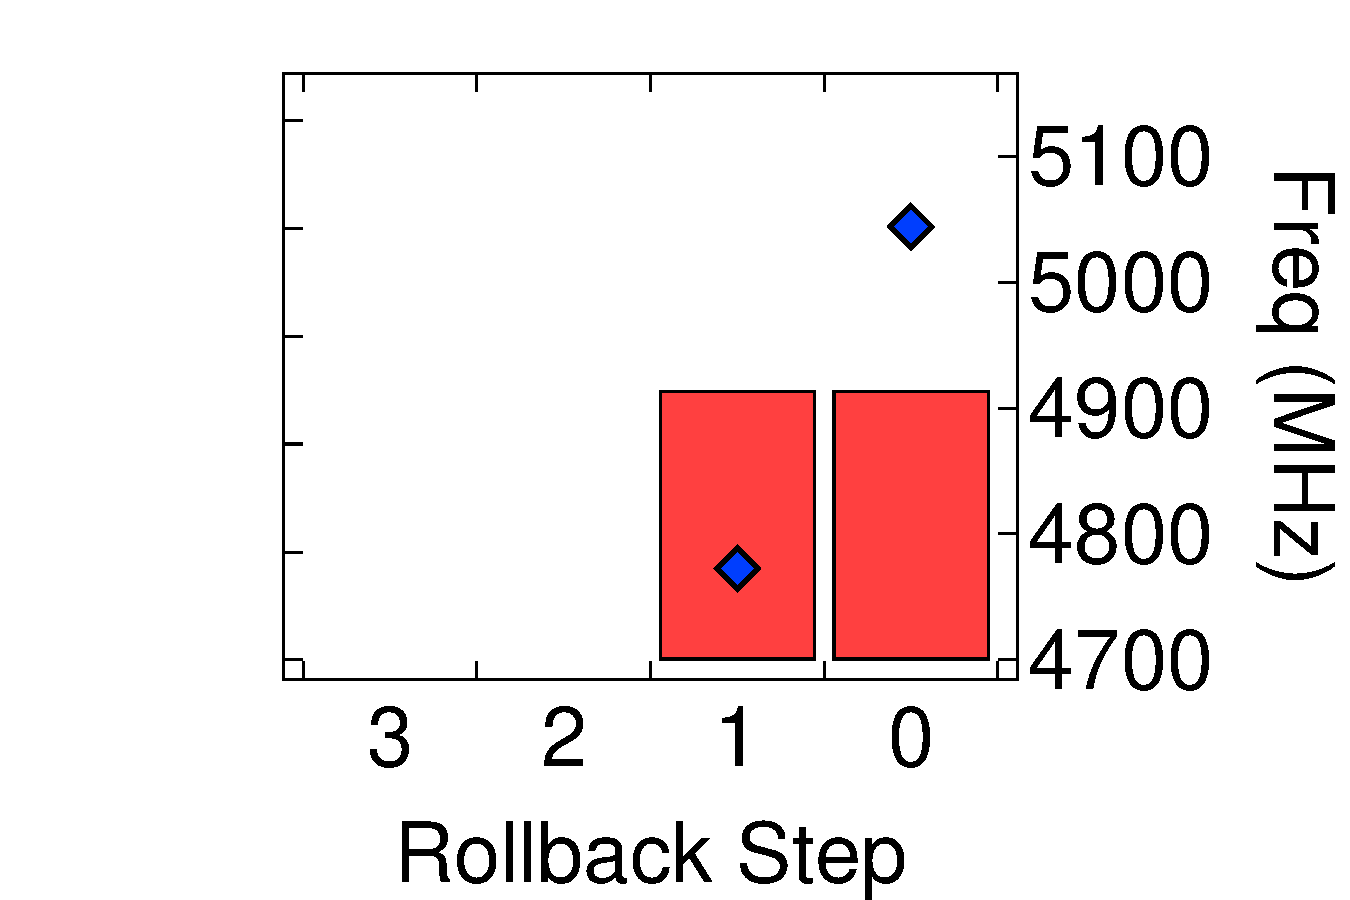
\includegraphics[trim=0 0 0 0,clip,width=.3\linewidth]{graphs/process/ubench-limit-dist/int-limit-dist-p1c7.pdf}
      }
    \caption{For 6 out of 16 cores, ATM configuration (i.e., CPM's inserted delay setting) needs to be rolled back from its idle limit in order for micro-benchmark (uBench) to run successfully. The 
    FP (\bench{daxpy}), MEM (\bench{stream}), and INT (\bench{coremark}) uBench have similar distribution of their pass config, indicating the core's mismatch between its reconfigured CPM timing measurement and its actual circuit speed. The other 10 cores not shown can run uBench safely at their idle limits.}
    \label{fig:ubench-limit-dist} 
\end{figure*}

%\begin{figure*}[t]
%      \subfloat[p0c3, \bench{daxpy}] {
%        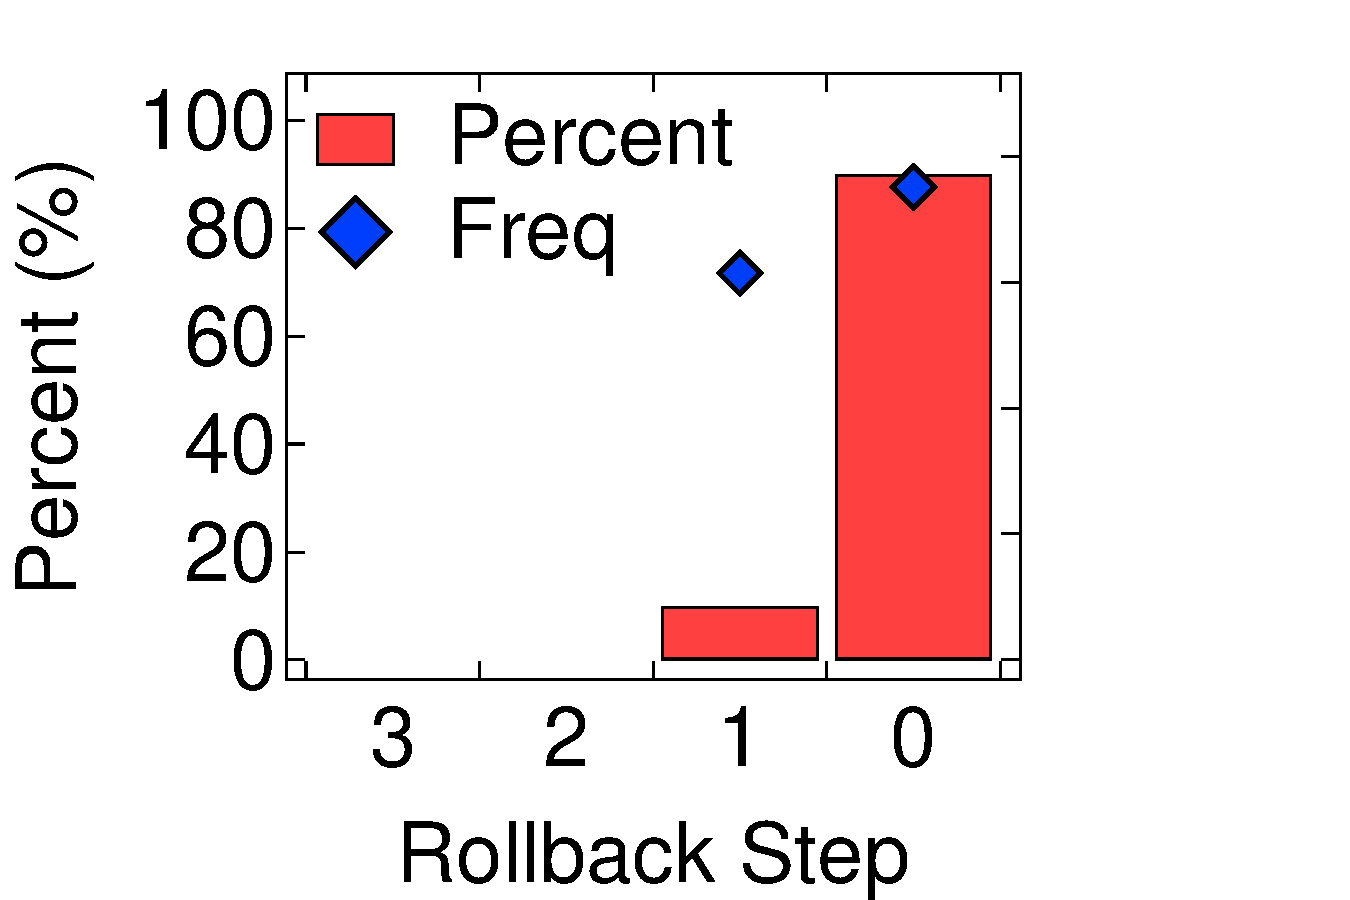
\includegraphics[trim=0 0 150 0,clip,width=.180\linewidth]{graphs/process/ubench-limit-dist/fp-limit-dist-p0c3.pdf}
%      }
%      \hfill
%      \subfloat[p0c4, \bench{daxpy}] {
%        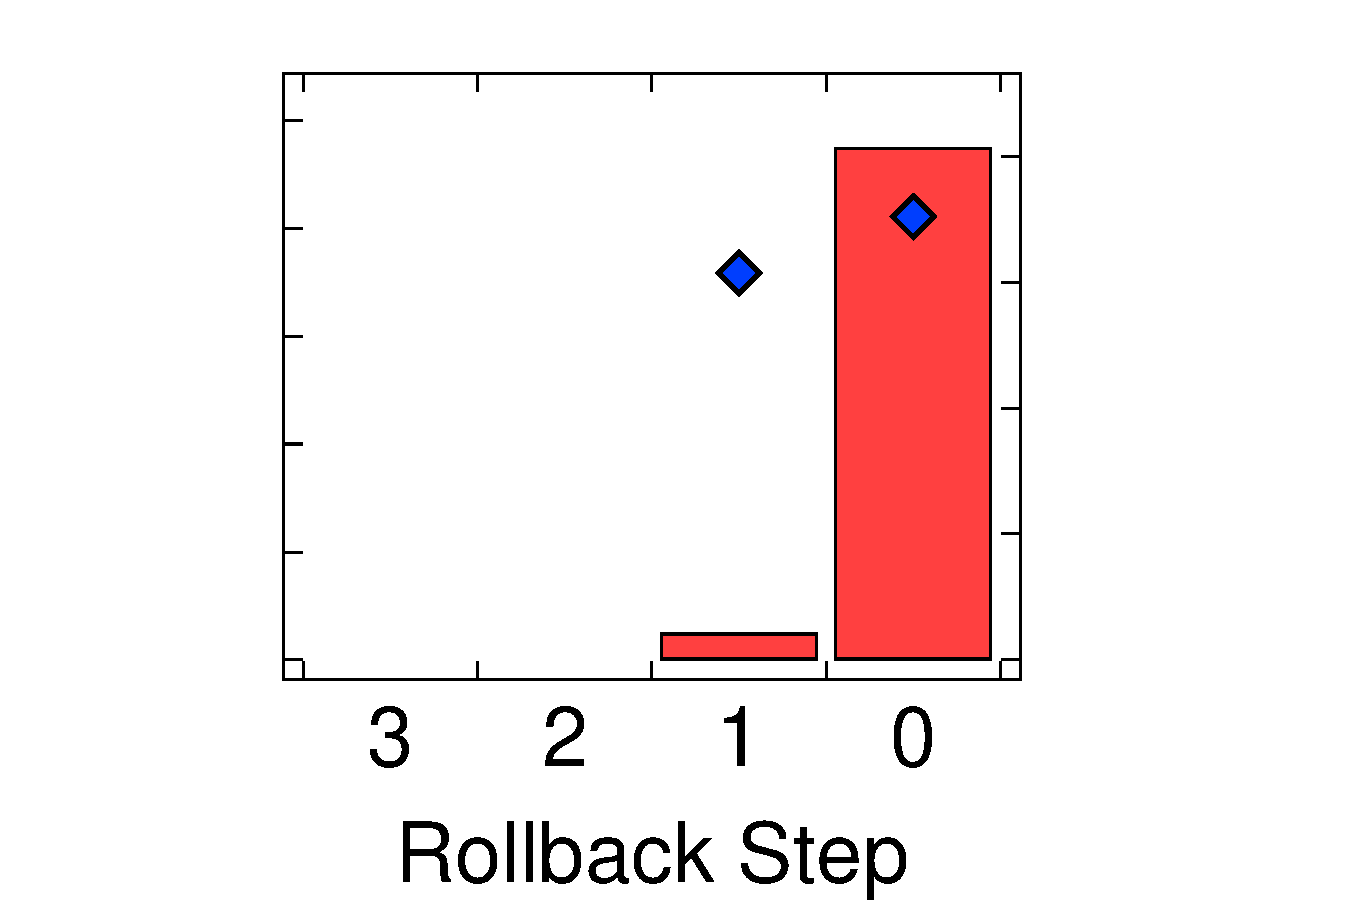
\includegraphics[trim=130 0 150 0,clip,width=.132\linewidth]{graphs/process/ubench-limit-dist/fp-limit-dist-p0c4.pdf}
%      }
%      \hfill
%      \subfloat[p1c3, \bench{stream}] {
%        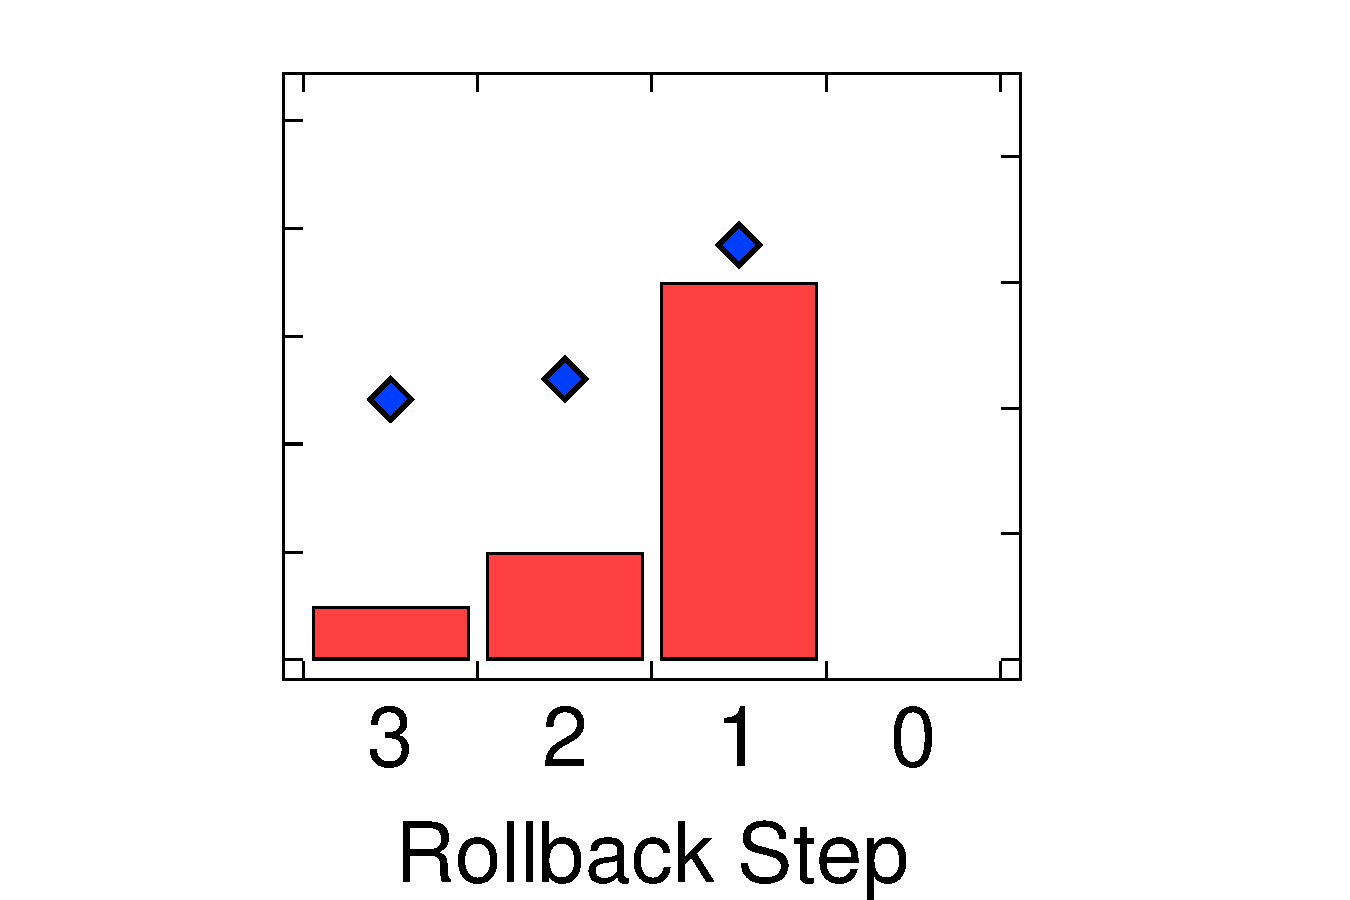
\includegraphics[trim=130 0 150 0,clip,width=.132\linewidth]{graphs/process/ubench-limit-dist/mem-limit-dist-p1c3.pdf}
%      }
%      \hfill
%      \subfloat[p1c4, \bench{stream}] {
%        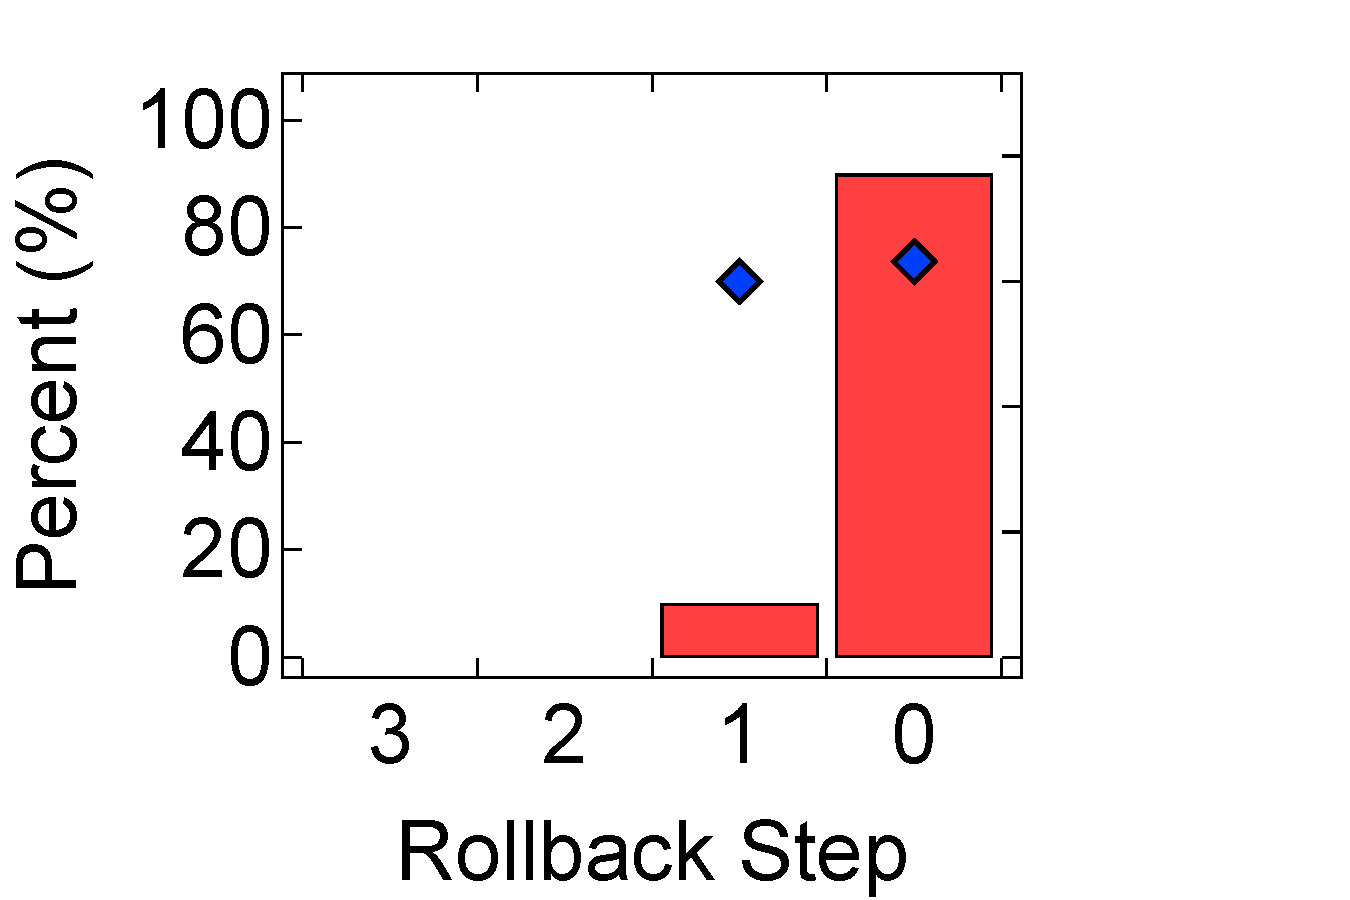
\includegraphics[trim=130 0 150 0,clip,width=.132\linewidth]{graphs/process/ubench-limit-dist/mem-limit-dist-p1c4.pdf}
%      }
%      \hfill
%      \subfloat[p1c5, \bench{coremark}] {
%        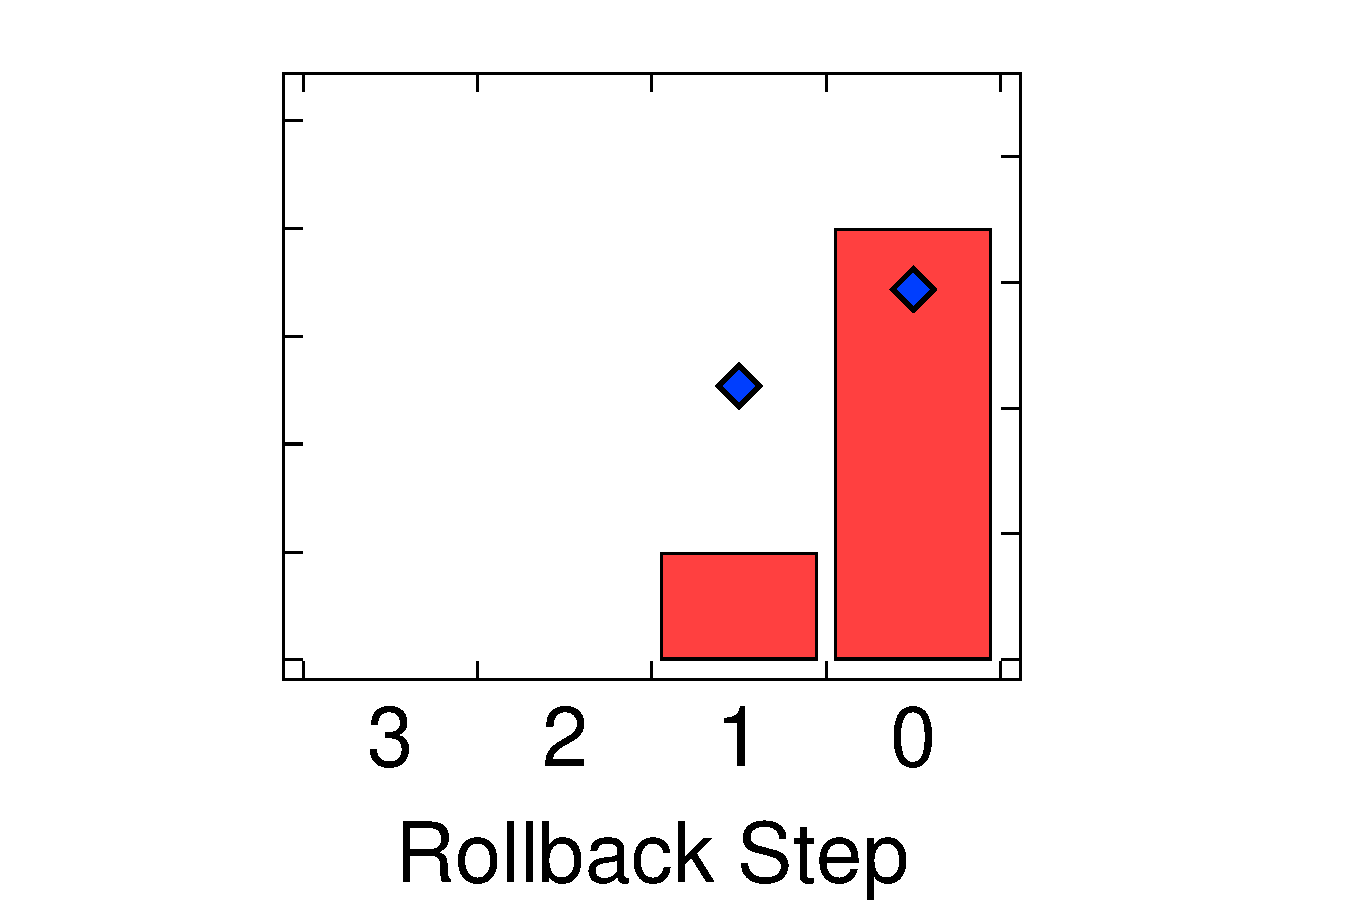
\includegraphics[trim=130 0 150 0,clip,width=.132\linewidth]{graphs/process/ubench-limit-dist/int-limit-dist-p1c5.pdf}
%      }
%      \hfill
%      \subfloat[p1c7, \bench{coremark}] {
%        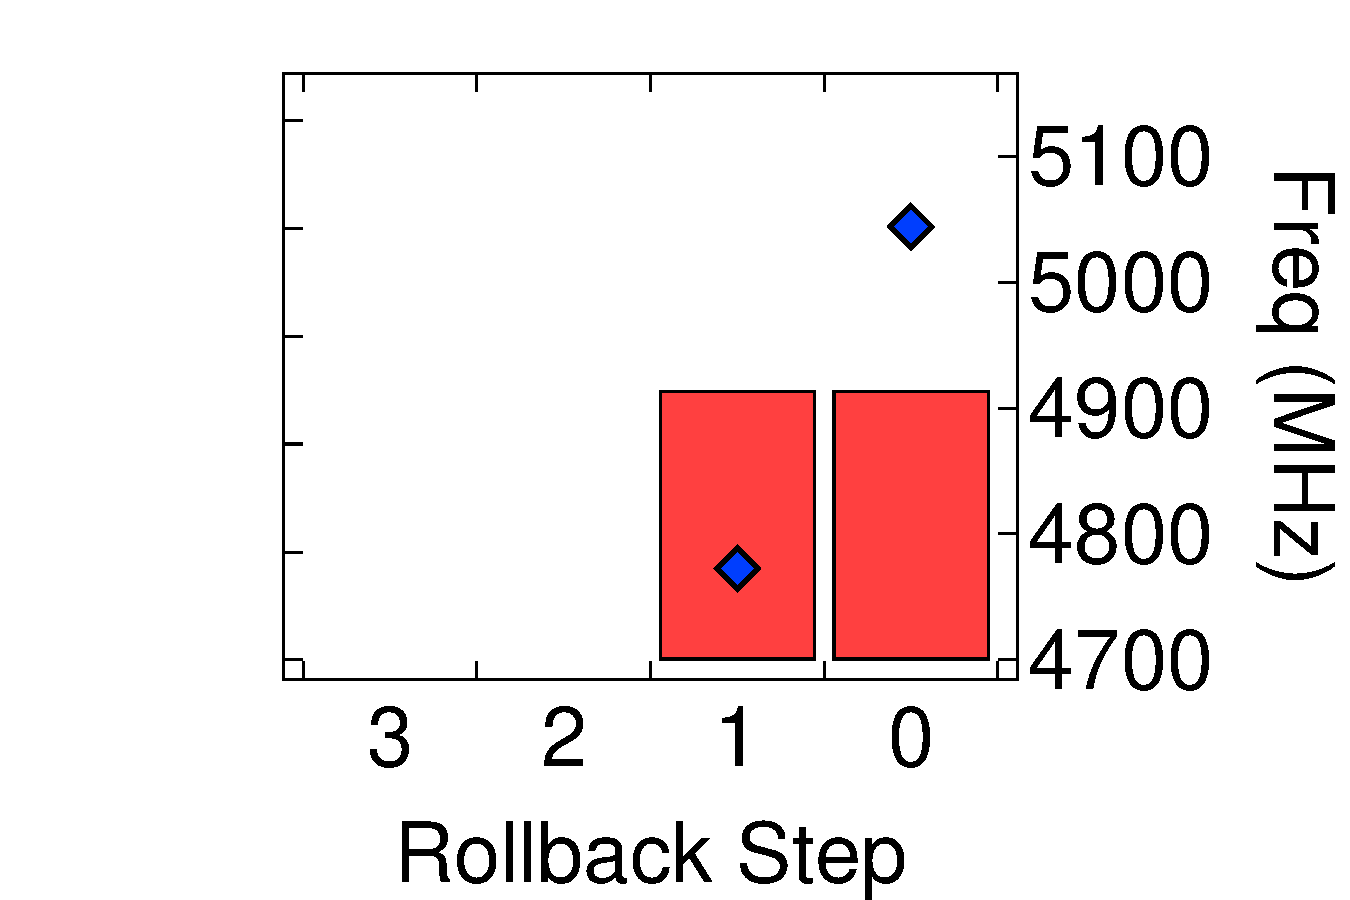
\includegraphics[trim=130 0 0 0,clip,width=.186\linewidth]{graphs/process/ubench-limit-dist/int-limit-dist-p1c7.pdf}
%      }
%    \caption{For 6 out of 16 cores, ATM configuration (i.e., CPM's inserted delay setting) needs to be rolled back from its idle limit in order for micro-benchmark (uBench) to run successfully. The 
%    FP (\bench{daxpy}), MEM (\bench{stream}), and INT (\bench{coremark}) uBench have similar distribution of their pass config, indicating the core's mismatch between its reconfigured CPM timing measurement and its actual circuit speed. The other 10 cores not shown can run uBench safely at their idle limits.}
%    \label{fig:ubench-limit-dist} 
%\end{figure*}

% \begin{figure*}[t]
%     \captionsetup[subfigure]{font=footnotesize}
%     \begin{subfigure}{.180\linewidth}
%         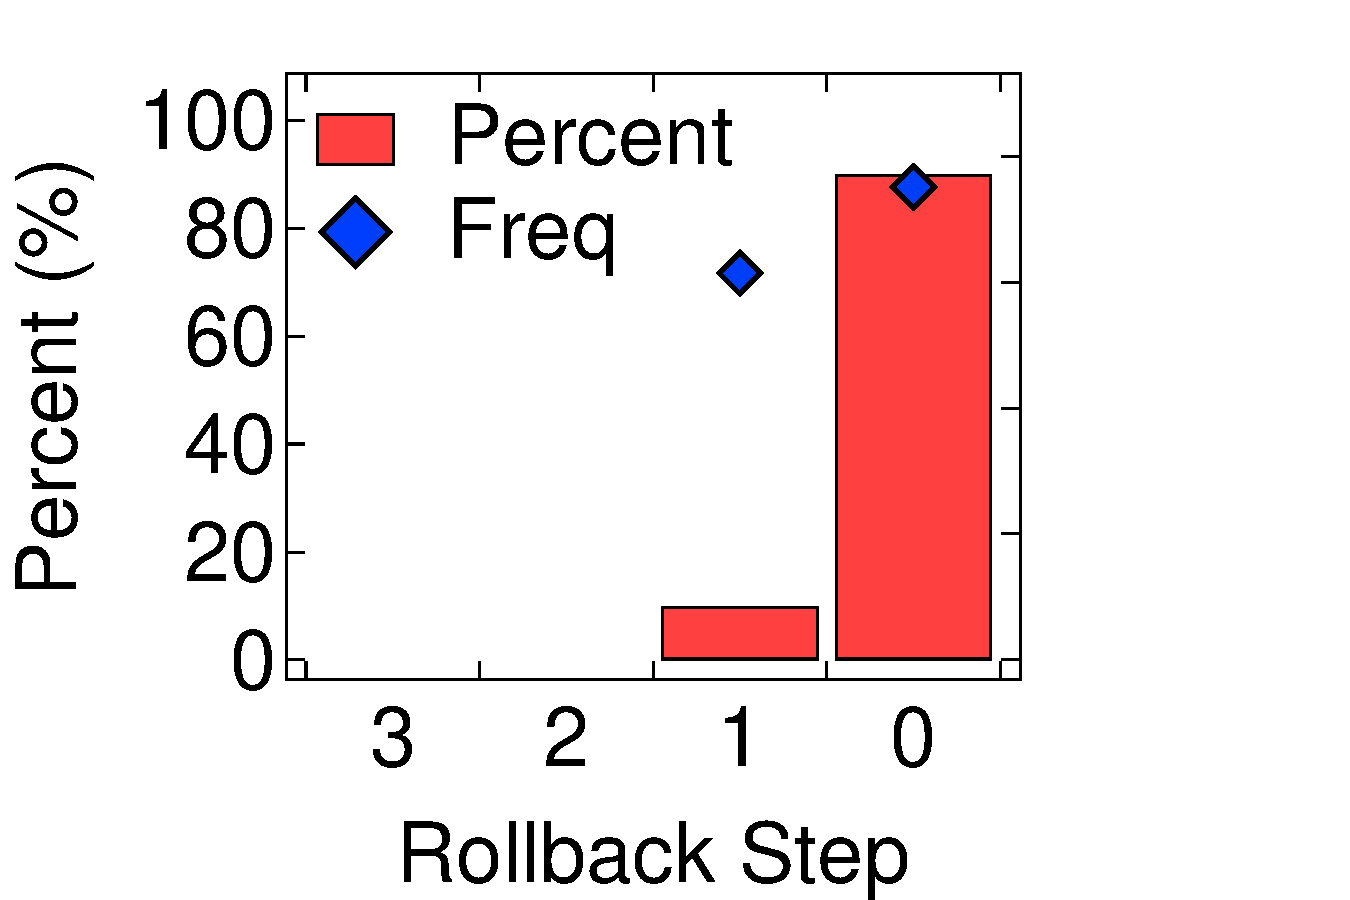
\includegraphics[trim=0 0 150 0,clip,width=\linewidth]{graphs/process/ubench-limit-dist/fp-limit-dist-p0c3.pdf}
%         \setlength{\abovecaptionskip}{-9pt}
%         \captionsetup{oneside,margin={23pt,0pt}}
%         \caption{P0C3, \\\bench{daxpy}}
%     \end{subfigure}
%     \hfill
%     \begin{subfigure}{.132\linewidth}
%         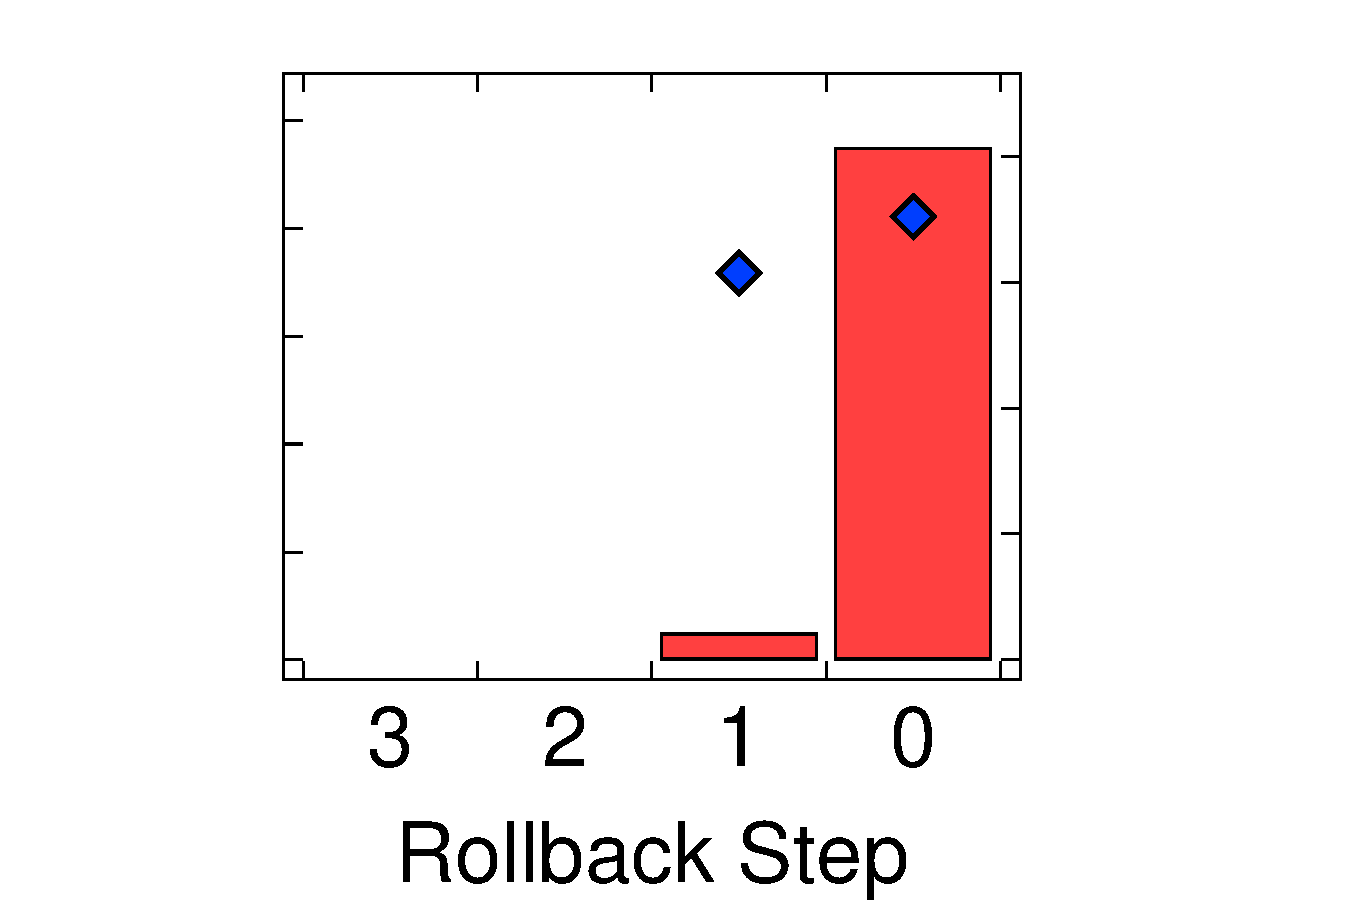
\includegraphics[trim=130 0 150 0,clip,width=\linewidth]{graphs/process/ubench-limit-dist/fp-limit-dist-p0c4.pdf}
%         \setlength{\abovecaptionskip}{-9pt}
%         \caption{P0C4, \\\bench{daxpy}}
%     \end{subfigure}
%     \hfill
%     \begin{subfigure}{.132\linewidth}
%         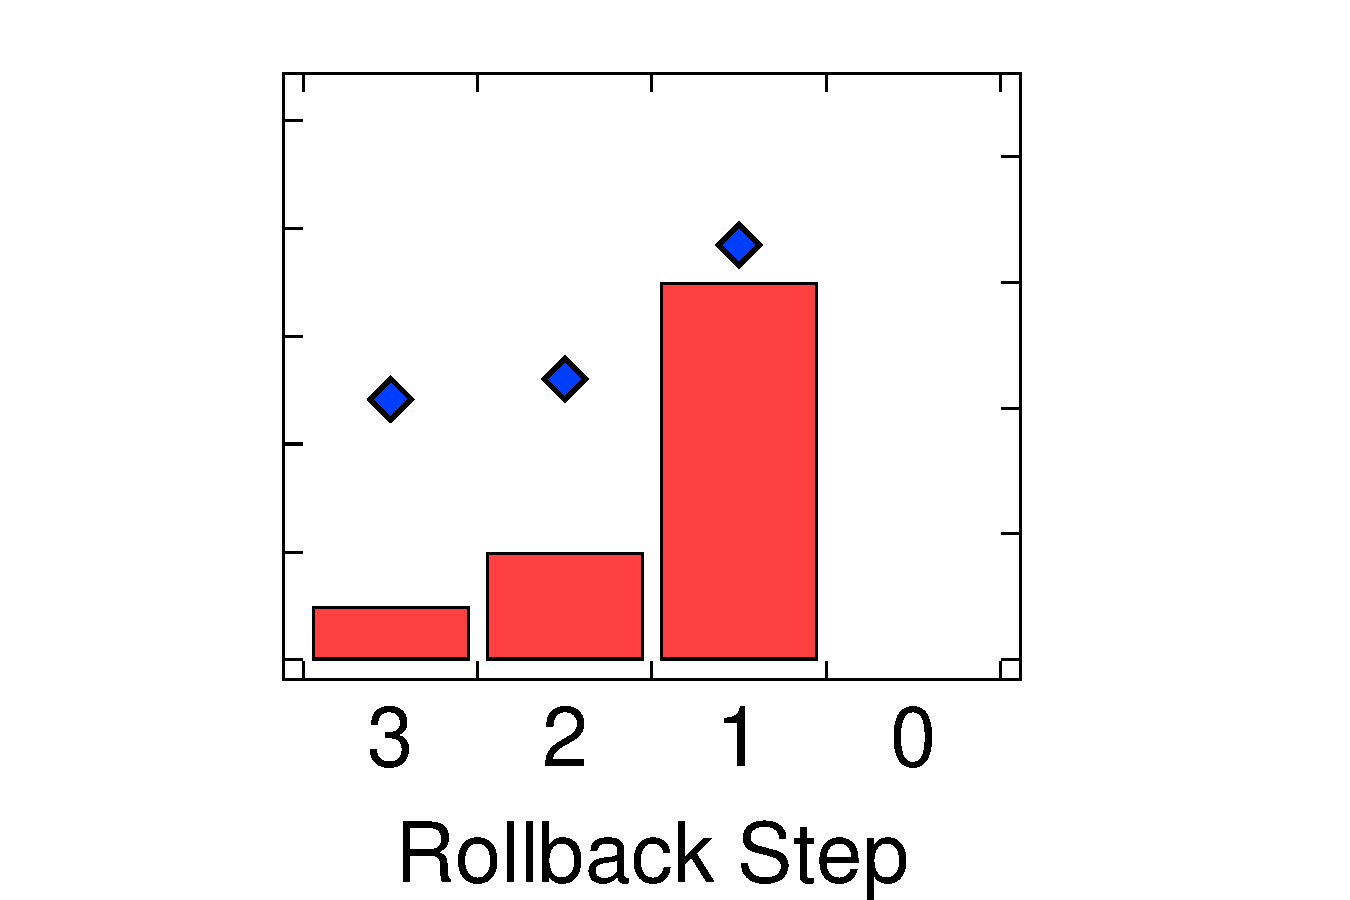
\includegraphics[trim=130 0 150 0,clip,width=\linewidth]{graphs/process/ubench-limit-dist/mem-limit-dist-p1c3.pdf}
%         \setlength{\abovecaptionskip}{-9pt}
%         \caption{P1C3, \\\bench{stream}}
%     \end{subfigure}
%     \hfill
%     \begin{subfigure}{.132\linewidth}
%         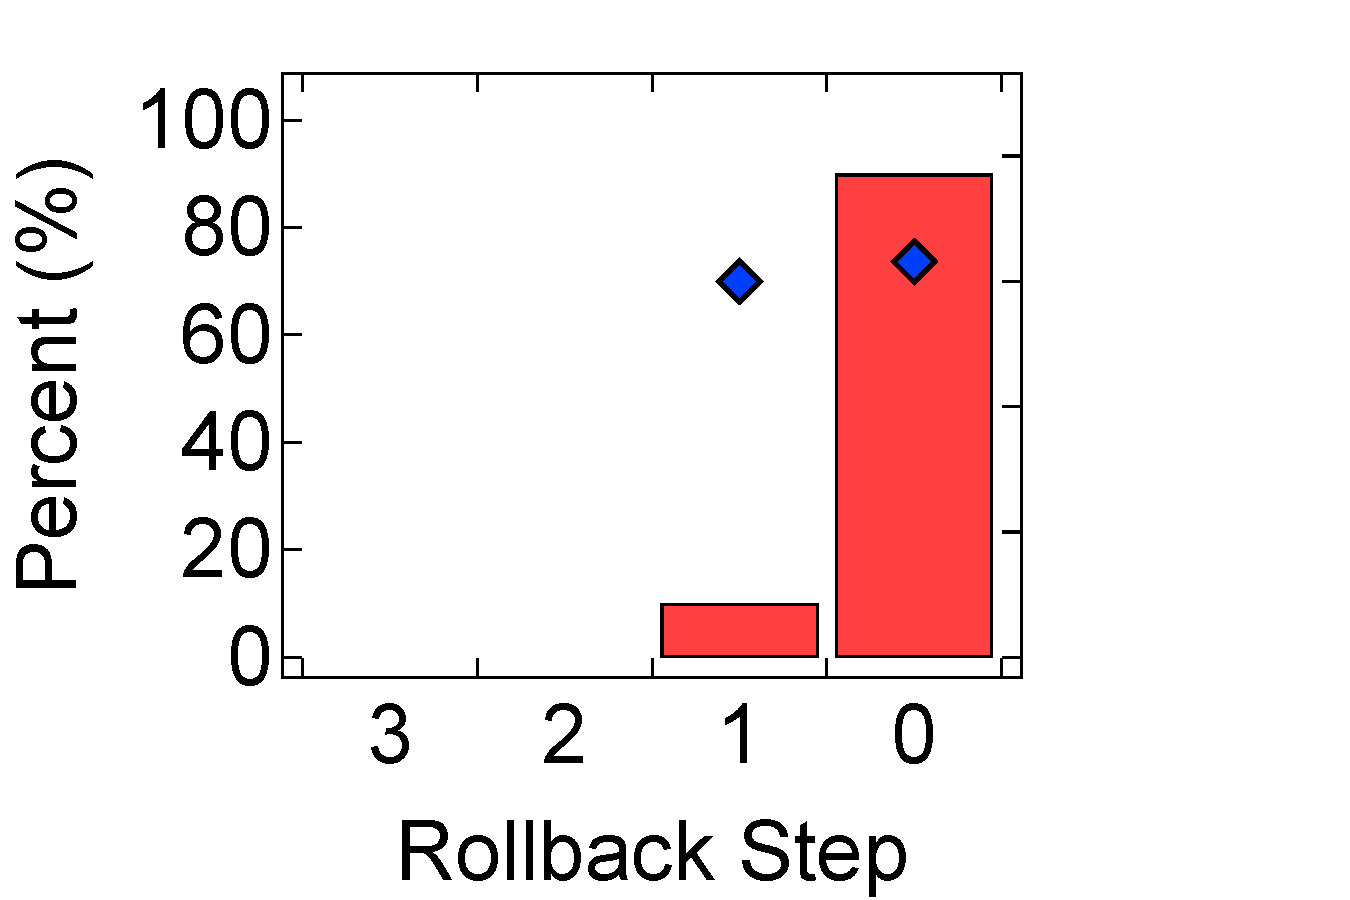
\includegraphics[trim=130 0 150 0,clip,width=\linewidth]{graphs/process/ubench-limit-dist/mem-limit-dist-p1c4.pdf}
%         \setlength{\abovecaptionskip}{-9pt}
%         \caption{P1C4, \\\bench{stream}}
%     \end{subfigure}
%     \hfill
%     \begin{subfigure}{.132\linewidth}
%         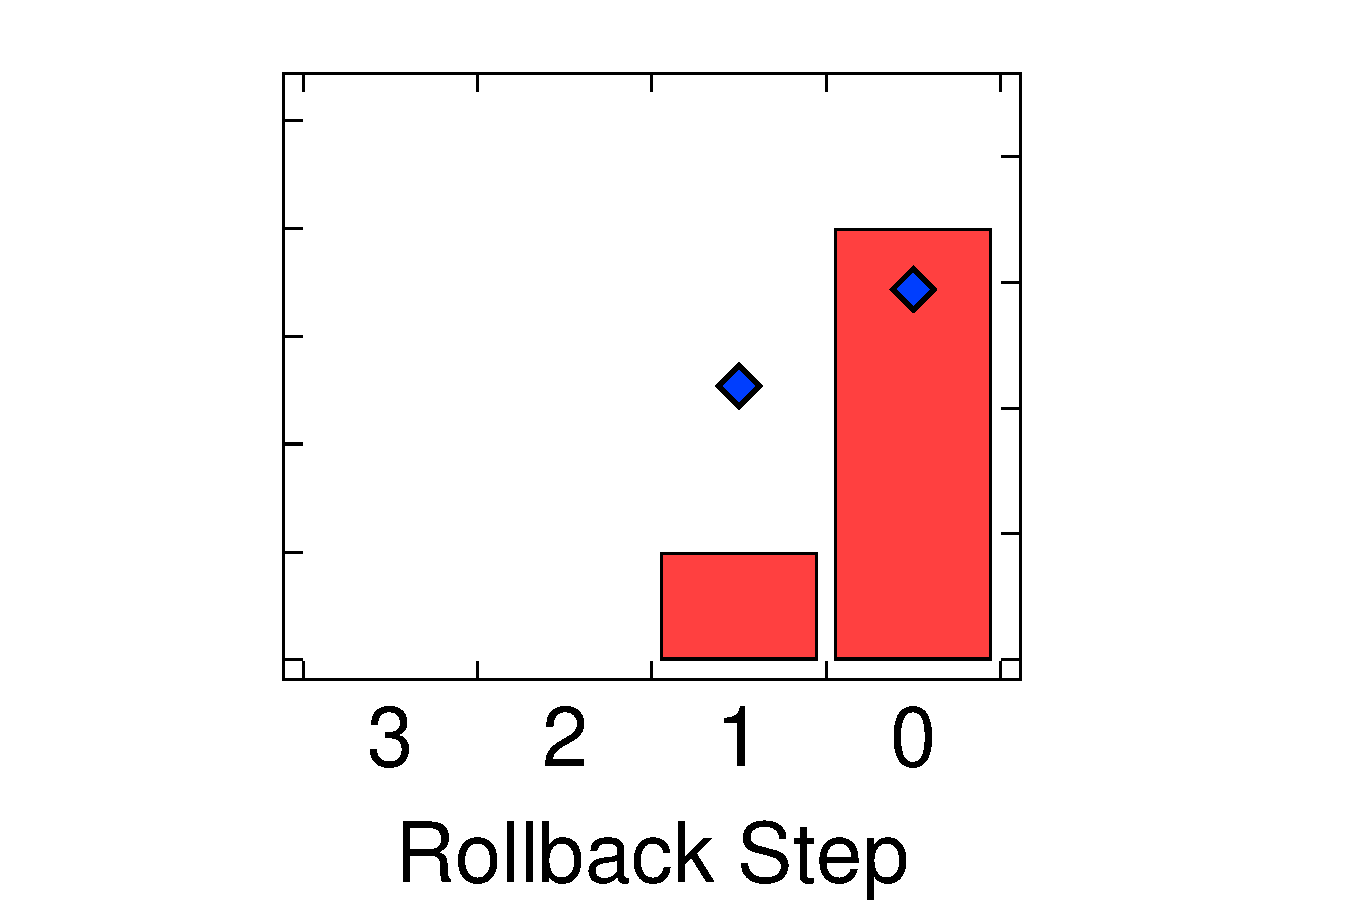
\includegraphics[trim=130 0 150 0,clip,width=\linewidth]{graphs/process/ubench-limit-dist/int-limit-dist-p1c5.pdf}
%         \setlength{\abovecaptionskip}{-9pt}
%         \captionsetup{oneside,margin={-4pt,0pt}}
%         \caption{P1C5, \\~~~~~\bench{coremark}}
%     \end{subfigure}
%     \hfill
%     \begin{subfigure}{.186\linewidth}
%         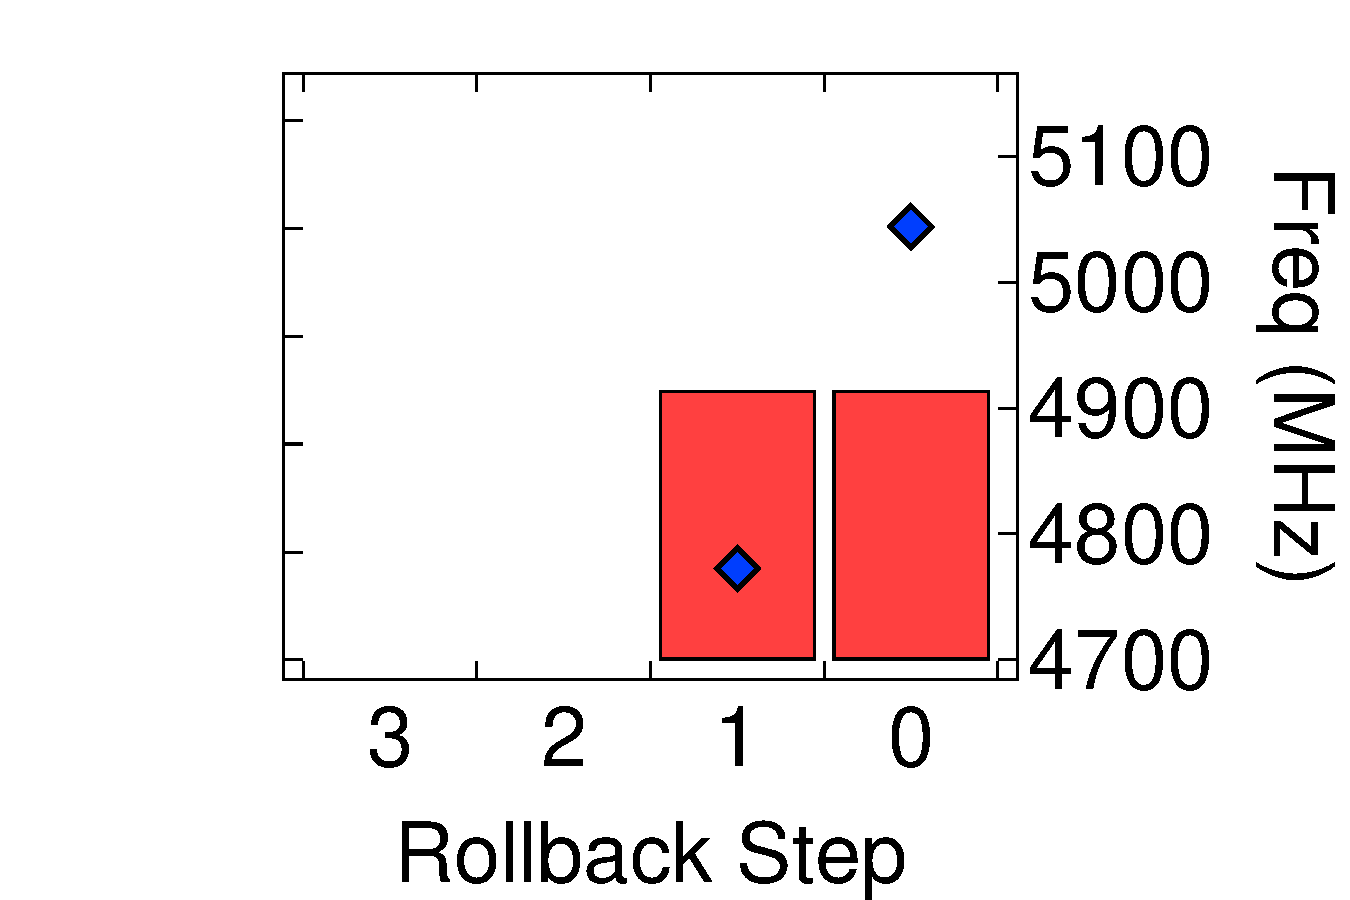
\includegraphics[trim=130 0 0 0,clip,width=\linewidth]{graphs/process/ubench-limit-dist/int-limit-dist-p1c7.pdf}
%         \setlength{\abovecaptionskip}{-9pt}
%         \captionsetup{oneside,margin={-4pt,27pt}}
%         \caption{P1C7, \\~~~~~\bench{coremark}}
%     \end{subfigure}
%     %\caption{For six cores, CPM inserted delay need to be rolled back from its idle limit for uBench to run correctly. The FP (\bench{daxpy}), MEM (\bench{stream}), and INT (\bench{coremark}) uBench have consistent behavior on the rolled back cores, indicating the core's idle limit is too aggressive and fails to capture some paths with long delay. The other 10 cores unshown can run uBench correctly at their idle limits.}
%     \caption{For the six cores shown above, CPM inserted delay needs to be rolled back from its idle limit for the uBench to run correctly, indicating the core's idle limit is too aggressive and fails to capture some long delay paths in the core.}
%     \label{fig:ubench-limit-dist} 
%     \vspace{-0.3cm}
% \end{figure*}
